\documentclass[10pt,preprint]{aastex}
% \documentclass[useAMS,usenatbib]{mn2e}
\usepackage{booktabs}
\usepackage{amsmath}
\usepackage{breqn}
\usepackage{cite,natbib}
% \usepackage{natbib}
\usepackage{verbatim}
\usepackage{epsfig}
\usepackage{cases}
\usepackage[section]{placeins}
\usepackage{graphicx, subfigure}
\usepackage{color}
\usepackage{amsmath}
\usepackage{float}
\floatplacement{figure}{H}

\newcommand{\logg}{log \emph{g}~}
\newcommand{\teff}{$T_{eff}$}
\newcommand{\prot}{$P_{rot}~$}

\newcommand{\ah}{$\hat{A}_n$}
\newcommand{\ph}{$\hat{P}_n$}
\newcommand{\ch}{$\hat{C}_n$}
\newcommand{\gh}{$\hat{G}_n$}
\newcommand{\yh}{$\hat{Y}_n$}
\newcommand{\teffh}{$\hat{T}_n$}
\newcommand{\chit}{$\chi^2$}

\newcommand{\feh}{[Fe/H]}
\newcommand{\dd}{\ensuremath{\,\mathrm{d}}}

% numbers
\newcommand{\nastero}{310}
\newcommand{\nprecise}{14~}
\newcommand{\ncluster}{282~}
\newcommand{\ntotal}{597~}
\newcommand{\ngarcia}{310~}
\newcommand{\ncooldwarfs}{23~}

% results
\newcommand{\gyroa}{0.310}
\newcommand{\aerrp}{0.03}
\newcommand{\aerrm}{0.01}
\newcommand{\gyron}{0.609}
\newcommand{\nerrp}{0.007}
\newcommand{\nerrm}{0.01}
\newcommand{\gyrob}{0.4361}
\newcommand{\berrp}{0.004}
\newcommand{\berrm}{0.005}
% (0.30958092212677002, 0.029399747848510849, 0.014372974634170532)
% (0.60851401090621948, 0.0074872469902038663, 0.014223098754882812)
% (0.43611901998519897, 0.0041089451313018888, 0.0053085982799530029)

% Notes for paper:

% Want to provide an estimate of the amount of intrinsic uncertainty on an age calculated with our method.
% The sun would be hard to detect in our survey.
% Notes - apparently asteroseismic ages are easier to derive for older stars!
% colour-mass relation is different for different compositions and this adds a level of systematic uncertainty.

\begin{document}

\title{Calibrating Gyrochronology using Kepler Asteroseismic targets}

\author{Ruth Angus$^1$, Suzanne Aigrain$^1$, Amy McQuillan$^2$, Daniel Foreman-Mackey$^3$,  William, J. Chaplin$^4$, Tsevi Mazeh$^2$}
\affil{$^1$Department of Physics, University of Oxford, OX1 3RH, UK}
\affil{$^2$School of Physics and Astronomy, Raymond and Beverly Sackler, Faculty of Exact Sciences, Tel Aviv University, 69978, Tel Aviv, Israel}
\affil{$^3$Centre for Cosmology and Particle Physics, New York University, New York, NY, USA}
\affil{$^4$School of Physics and Astronomy, University of Birmingham, Edgbaston, Birmingham, B15 2TT, UK}

\begin{abstract}
\label{abs}

Measuring ages for intermediate and low-mass stars on the Main Sequence (MS) is challenging but important for a wide range of studies, from Galactic dynamics to stellar and planetary evolution.
Among the available methods, gyrochronology is a powerful one because it requires knowledge of only the star's mass (or effective temperature, or colour) and its rotation period.
However, it is not well calibrated at late ages and suffers from large uncertainties.
Asteroseismology provides age measurements for some of the brightest stars observed by Kepler.
% We measured the photometric rotation periods of 153 stars with asteroseismic ages in order to calibrate the gyrochronology relations and improve upon current methods of measuring the ages of MS field stars. %pchange
We use rotation periods measurements of \nastero stars with asteroseismic ages, \ncluster cluster stars and 5 field stars (including the Sun) with precise age measurements to calibrate the gyrochronology relations.
Advanced statistical methods are used to model the relationship between rotation period, age and colour while accounting for measurement uncertainties in all three quantities.
Our sample includes both MS stars and subgiants, and straddles the Kraft break (only MS stars cooler than the Kraft break, $\sim$ 6250 K, are expected to follow gyrochronology relations); and this must be taken into account when modelling the data.
Our method has been applied to the extended sample of published rotation periods for stars with reliable age measurements.
It enables us to estimate an age for any cool MS star with a measured period and colour, along with an associated uncertainty that reflects both measurement errors and the intrinsic scatter in the gyrochronology relations.
Formal uncertainties on stellar ages calculated with this new gyrochronology relation will typically be of order ...\%.
We find that this sample of asteroseismic stars does not fall neatly onto the mass-period-age plane---there is a significant level of intrinsic scatter.
It is currently unclear whether this scatter is a manifestation of noisy data or if stars cease to be well described by gyrochronology in general, past a certain age.
Uncertainties on the ages of this asteroseismic sample are of order 35\%---advancements in age measurement precision anticipated over the coming months will be key for our understanding of the applicability of gyrochronology.

\end{abstract}

\section{Introduction}
\label{intro}
\subsection{Dating methods for field stars}

Many fields of astronomy rely on precise age measurements of Main Sequence (MS) stars.
Unfortunately, the ages of MS stars are notoriously difficult to measure---observable stellar properties evolve slowly on the MS and even with high precision measurements of spectroscopic properties, ages often cannot be determined accurately to within 20\% \citep{Soderblom2010}.
Cluster stars have some of the most reliable and precise age measurements currently available, where isochrones can be fitted to a coeval population with a range of masses, resulting in age measurements with uncertainties often as low as 10\%.
Isochronally derived field star ages on the other hand, are much less precise than this and often have uncertainties of order 50\% or more.
Demand for age estimates of planet-hosting stars is high, but faint stars observed by Kepler are often expensive or impractical spectroscopic targets.
Where high resolution spectra are unavailable, or an independantly derived age measurement is required, gyrochronology can be extrememly useful.
Gyrochronology is a dating method that utilises the predictable rotation period evolution of intermediate mass, MS stars.
It requires only knowledge of the rotation period---which is often easily extracted from Kepler light curves, and mass (or appropriate proxy) of a star.
The current gyrochronology relations are entirely empirically calibrated and still need refining at large stellar ages.
Kepler data provides the perfect opportunity to calibrate gyrochronology at late ages---it not only provides the means to measure surface rotation of thousands of stars, it also provides new age estimates for hundreds of stars via asteroseismology.
We use new asteroseismic age measurements to improve the gyrochronology relations at late ages.

\subsection{Gyrochronology}

Mass loss via a magnetised stellar wind causes magnetic breaking of MS stars \citep{Weber1967}.
A dynamo-driven magnetic field, generated at the tachocline---the interface between radiative and convective zones---locks the stellar wind to the surface of the star.
The stellar wind corotates with the stellar surface out to the Alfv\'{e}n radius, at which point it decouples and angular momentum is lost from the star.
The strength of the magnetic field at the surface, and therefore the rate of angular momentum loss, is inversely proportional to rotation period \citep{Kawaler1988}.
Due to this dependence, although stellar populations are born with a range of rotation periods, the rapid rotators rapidly lose angular momentum and rotation periods converge onto a unique sequence.
The timescale for convergence is around the age of the Hyades: 650 Myrs (\citealt{Radick1987}, \citealt{Irwin2009}).
After this time rotation periods are \emph{independent} of their initial values.
The form of angular momentum evolution described above and calibrated in this article can only be applied to F, G and K MS stars.
Fully convective M dwarfs have a different dynamo-driven magnetic field.
Their rotation periods evolve over extremely long timescales and they often do not converge onto the mass-period-age plane, even after several Gyrs.
Stars with effective temperatures $\gtrsim$ 6250 K have shallow convective zones - they are almost fully radiative - and, again, they have a different dynamo-driven magnetic field \citep{Kraft1967}.
These massive stars retain their initial rotation period throughout their brief MS lifetimes and are therefore not suitable gyrochronology targets.

The rate of rotation period decay for intermediate mass MS stars was first quantified by \citet{Skumanich1972}, who observed rotation period, lithium abundance and chromospheric activity to be proportional to $\mathrm{Age}^{\frac{1}{2}}$.
% \citet{Skumanich1972} quantified the decay of stellar activity and rotational period as proportional square-root of age.
Later, \citet{Noyes1984_2} added a mass dependence was added to the period-activity-age relation: more massive stars were observed to spin down more slowly.
The term `gyrochronology' was coined by \citet{Barnes2003} who proposed an empirically motivated functional form for the relation between period, colour and age,
\begin{equation}
P = A^n \times a(B-V-0.4)^b,
\label{eq:Barnes2007_2}
\end{equation}
where $P$ is rotation period (in days), $A$ is age (in Myr), $B$ and $V$ are B and V band magnitudes respectively and $a$, $b$, and $n$ are constants.
The discontinuity in the period-colour relation was set to be 0.4.

This gyrochronology relation was calibrated using open clusters.
Clusters are invaluable calibration tools, however unfortunately the majority of nearby clusters are young---there is a significant dearth of precisely measured ages for old stars and it is for this reason that the current gyrochronology relations are poorly calibrated at late ages.
\citet{Barnes2007} used 8 young open clusters, aged between 30 and 650 Myrs to calibrate the dependence of rotation period on mass, and the Sun to calibrate the dependence on age.
Best-fit values of $n$, $a$ and $b$, reported in \citet{Barnes2007} are tabulated in \ref{tab:constants}.
This relation was further calibrated by \citet{Mamajek2008} using updated rotation period and age measurements of stars in open clusters $\alpha$ Per \citep{Prosser1995}, Pleiades (\citealt{Prosser2005}; \citealt{Krishnamurthi1998}), M34 \citep{Meibom2011_M34}, and Hyades (\citealt{Radick1987}; \citealt{Prosser1995}; \citealt{Radick1995}; \citealt{Paulson2004}; Henry, priv. comm.).
Once again, the Sun was used as an age anchor---a single data point specifying the shape of the period-age relation.
Whereas \citet{Barnes2007} fixed the position of the `colour discontinuity' at 0.4, \citet{Mamajek2008} allow it to be a free parameter in their model, calling it `$c$'.
The values of $n$, $a$ and $b$, resulting from their fit are tabulated in \ref{tab:constants}.
% \citet{Mamajek2008} only retained fits that reproduced the rotation period of the Sun to within 0.1 days.
% This approach relies on the Copernican principle---they assume that the Sun is a typical rotator for its mass and age.
% If this assumption is invalid (it is, at least, not well motivated) then their resulting gyrochronological relation will incorrectly predict ages of stars older than the Hyades.
In both of these studies a minimum \chit fitting approach was used.
Simple minimum \chit fitting relies on the assumption that uncertainties are Gaussian, which may not always be the case (although could be a reasonable approximation) and only takes observational uncertainties on the dependent variable into account.
As described later in this article, we adopt a fitting method that properly accounts for observational uncertainties on all three variables: colour, period and age.

\begin{deluxetable}{lccc}
\label{tab:constants}
\tablewidth{0pc}
\tablecaption{Values of a, b, c \& n in \citet{Barnes2007} and \citet{Mamajek2008} and this work.}
\tablehead{
\colhead{Parameter}&
\colhead{\citet{Barnes2007}}&
\colhead{\citet{Mamajek2008}}&
\colhead{This work}}
% 2.726685106754302979e-01 7.484385967254647554e-03 1.548099517822265625e-02
% 6.197596788406372070e-01 3.800292015075590335e-03 4.473507404327392578e-03
% 4.090114831924438477e-01 2.897063493728646577e-03 3.478863596916198508e-02
\startdata
a & $0.7725 \pm 0.011$ & $0.407 \pm 0.021$ & $\gyroa^{+\aerrp}_{-\aerrm}$ \\
b & $0.601 \pm 0.024$ & $0.325 \pm 0.024$ & $\gyrob^{+\aerrp}_{-\berrm}$\\
c & $0.4$ & $0.495 \pm 0.010$ & $0.45$ \\
n & $0.5189 \pm 0.0070$ & $0.566 \pm 0.008$ & $\gyron^{+\nerrp}_{-\nerrm}$\\
\enddata
\end{deluxetable}

\subsection{Asteroseismic ages}
\label{sec:asteroseismic_targets}

Acoustic (pressure) mode oscillations produce periodic luminosity variations on timescales of $\sim$ 5 minutes in Solar-like stars.
These oscillations are detectable in short-cadence Kepler data---a fourier transform of the time series reveals a series of narrow peaks at discrete frequencies, overtones of high radial order, $n$.
The frequency spacing, (or large frequency separation, $\Delta\nu_{nl} = \nu_{n+1l}-\nu_{nl}$) between consecutive overtones, $n$, of the same degree, $l$, is a fundamental asteroseismic observable.
The series of peaks in the Fourier transform is modulated by a gaussian envelope, the maximum of which is another fundamental asteroseismic observable, $\nu_{\mathrm{max}}$.
These two fundamental asteroseismic parameters together with effective temperature can be used, via the scaling relations below, to derive stellar masses and radii.

\begin{equation}
\frac{\Delta\nu}{\Delta\nu_{\odot}} \approx \sqrt{\frac{M/M_{\odot}}{R/R_{\odot}^3}}
\label{eq:delta_nu}
\end{equation}

\begin{equation}
\frac{\nu_{\mathrm{max}}}{\nu_{\mathrm{max},\odot}} \approx \frac{M/M_{\odot}}{(R/R_{\odot})^2\sqrt{(T_{\mathrm{eff}}/T_{\mathrm{eff},\odot})}}
\label{eq:delta_nu}
\end{equation}

In particular, the mean large frequency separation, $\Delta\nu$ is proportional to the mean stellar density---since stellar density changes over the MS lifetime of a star, this parameter enables us to measure ages.

% \citet{Chaplin2013} calculated the ages of 505 Kepler targets using the above scaling relations.
% A grid-based approach was used to measure stellar properties: values of $\Delta\nu$ were calculated for each R and M on the grid and compared with the observed $\Delta\nu$.
% Ages quoted in \citet{Chaplin2013} are the combined result of six different grid-based model pipelines.
% The uncertainties on the ages reflect discrepancies between results obtained using different sets.
% Two sets of effective temperatures were used: one was derived using an Infra-Red Flux Method (IRFM) calibration (\citealt{Casagrande2010}, \citealt{SilvaAguirre2012}) and the other from a recalibration of the SDSS griz filter KIC photometry by \citet{Pinsonneault2012} using Yale Rotating Stellar Evolution Code (YREC) models \citep{Demarque2004}.
% We use the second set of temperatures since they are slightly more precise, however our analysis is relatively insensitive to this choice.
% % test: is our analysis sensitive to this choice?
%
% The asteroseismic ages in \citet{Chaplin2013} have typical uncertainties of $\sim$ 35\%; however, it will be possible to derive more precise ages for some of these stars.
% By measuring the frequency of each oscillation mode individually, not just the mean large serparation, one can build up a density profile of the star and provide a tighter constraint on its age.
% Ages derived from individual oscillation mode measurements can have uncertainties as small as 10\% (\citet{Brown1994}, \citet{SilvaAguirre2013}), however measuring frequencies for individual oscillation modes is a manual process and can only be applied in the highest signal-to-noise cases.
% \citet{Chaplin2013} predict that around 150 of the 505 stars will be suitable for this individual oscillation mode treatment.
% We obtained precise ages for 42 stars from \citet{Metcalfe2014}, modelled with the Asteroseismic Modeling Portal (AMP), with effective temperatures and metallicities from \citet{Bruntt2012}.
% % Of the 42 stars in \citep{Metcalfe2014}, we only integrate the `simple stars' (cool dwarfs) into our sample---we ignore the `F stars' and `mixed mode' (subgiant) stars as these are not expected to follow the simple gyrochronology relation.
% % {\color{red} Shouldn't I include these to be consistent?}

\section{Observations}
\label{sec:data}

\subsection{Ages}
\label{sec:ages}

The ages of 505 Kepler dwarfs and giants were published in \citet{Chaplin2013}.
They used a grid-based approach to measure stellar properties: values of $\Delta\nu$ were calculated for each R and M on the grid and compared with the observed $\Delta\nu$.
Ages quoted in \citet{Chaplin2013} are the combined result of six different grid-based model pipelines and the uncertainties on the ages reflect discrepancies between results obtained using different sets.
Two sets of effective temperatures were used: one was derived using an Infra-Red Flux Method (IRFM) calibration (\citealt{Casagrande2010}, \citealt{SilvaAguirre2012}) and the other from a recalibration of the SDSS griz filter KIC photometry by \citet{Pinsonneault2012} using Yale Rotating Stellar Evolution Code (YREC) models \citep{Demarque2004}.
We use the IRFM temperatures since they are less dependent on metallicity, which is not well constrained for the asteroseismic sample, and their uncertainites are more conservative.
Our analysis however, is relatively insensitive to this choice.
87 stars in the asteroseismic catalogue have spectroscopic measurements of \teff and \logg which were incorporated where possible.
In order to produce a relation that predicts the age of a star using only observable properties, we chose to convert \teff to B-V for the asteroseismic sample using the relation of \citet{Sekiguchi2000}.
This conversion adds an extra element of noise to our data since the metallicities provided for the asteroseismic stars are simply an average value for the field: $0.2\pm0.3$ dex (e.g. see \citealt{Silva_Aguirre}) however, since the age uncertainties dominate this analysis we do not expect this to have a significant impact on our results.

The asteroseismic ages in \citet{Chaplin2013} have typical uncertainties of $\sim$ 35\%; however, for some of these stars it will be possible to derive more precise ages.
By measuring the frequency of each oscillation mode individually, not just the mean large serparation, one can build up a density profile of the star and provide a tighter constraint on its age.
Ages derived from individual oscillation mode measurements can have uncertainties as small as 10\% (\citet{Brown1994}, \citet{SilvaAguirre2013}), however measuring frequencies for individual oscillation modes is a manual process and can only be applied in the highest signal-to-noise cases.
\citet{Chaplin2013} predict that around 150 of the 505 stars will be suitable for this individual oscillation mode treatment.
We obtained precise ages for 42 stars from \citet{Metcalfe2014}, modelled with the Asteroseismic Modeling Portal (AMP), with effective temperatures and metallicities from \citet{Bruntt2012}.
Of the 42 stars in \citet{Metcalfe2014}, we only integrate the `simple stars' (cool dwarfs) into our sample---we ignore the `F stars' and `mixed mode' (subgiant) stars as these are not expected to follow the simple gyrochronology relation.

\subsection{Rotation Periods}
\label{sec:rotation_periods}

The Kepler light curves of the 505 asteroseismic targets display quasi-periodic variations on timescales corresponding to rotational periods of the stars.
Flux variations are produced by active regions on the stellar surface, rotating in and out of view.
% In order to measure periodic signals in the light curves we used the auto-correlation function (ACF) method, developed by \citet{McQuillan2013}.
Rotation periods for \ngarcia stars are published in \citet{Garcia2014} who used a combination of autocorrelation and wavelet transforms to measure surface rotation of the Kepler asteroseismic targets.
An autocorrelation function describes the self-similarity of a light curve at a range of lags and the highest peak in the ACF (usually also the first peak) is centered on the dominant periodic signal in the time series.
As an alternative to the standard Fourier decomposition and least-squares fitting of sinusoidal models \citep{Zechmeister}, autocorrelation is better suited to signals that are not sinusoidal or strictly periodic and is more effective at distinguishing a true signal from its harmonics and sub-harmonics.
For a more detailed description of the advantages of the ACF method over sine-fitting periodograms, see \citet{McQuillan}.
A Wavelet Power Spectrum (WPS) is computed by calculating the correlation between the data and the Mother wavelet at a range of frequencies.
Unlike sine fitting periodograms and ACFs it is sensitive to the location of signals.
% \citet{Garcia2014} use a combination of a WPS method and an ACF method to measure the surface rotation periods of Kepler asteroseismic stars.
A wavelet power spectrum of each light curve calculated, using a Morlet mother wavelet, and then projected along the period axis to produce a global wavelet power spectrum (GWPS).
This projection reinforces the height of the fundamental peak and reduces those of the harmonic and sub-harmonic peaks.
The GWPS method is outlined in detail in \citep{Mathur2014}.
A Gaussian profile is fitted to each peak in the GWPS.
The highest peak is selected as the rotation period and the uncertainty quoted on the period measurement the half width of half maximum (HWHM) of the Gaussian profile.
The GWPS provides an indication of whether a persistent sinusoidal pattern, commensurate with star spot modulation, is present in the light curves, allowing the authors to eliminate signals produced by light curve glitches.
Rotation periods are only reported for stars with light curves displaying at least four full sinusoidal modulations.
Two versions of the detrended Kepler light curves were used in their analysis: Simple Aperture Photometry (SAP) data \citep{Thompson2013}, detrended using the Kepler Asteroseismic Data Analysis and Calibration Software (KADACS) \citep{Garcia2011} and long cadence Pre-Data Conditioning Maximum \emph{a Posteriori} (PDC-MAP) data, available for download through MAST.
The PDC-MAP data are the product of an initial systematics removal process applied by the Kepler team, in which large-scale linear trends are removed in order to improve planet transit search and modelling capability (\citet{Smith_2012}, \citet{Stumpe_2012}).
PDC-MAP data are not, however, optimised to preserve stellar variability: in particular, periodic signals longer than around 20 days are reduced in power.
Additionally, light curves still contain large systematic features, such as the exponential decays that appear after telescope shutdowns, which affect period measurement precision.
For this reason, \citet{Garcia2014} chose to use their own set of KADACS light curves in addition to the PDC-MAP data.
The GWPS and ACF methods were applied to both PDC-MAP and KADACS light curves and at least two of the four possible light curve and method combinations were required return rotation periods consistent to within 20\%.
A visual check was then performed to confirm that the measured period is representative of the timescale of variability in the light curves.
The final reported rotation periods were those measured from KADACS light curves using the GWPS method with HWHM uncertainties.
Of the 505 targets in the original sample, \nastero rotation periods were reliably measured using the above process.
Of those \nastero, \nprecise of them have precise asteroseismic ages from AMP modelling.

The asteroseismic sample covers a large range of ages (see figure \ref{fig:p_vs_a}), however it does not provide good mass coverage across the entire range.
Few stars have temperatures below 6000 K (B-V $\sim$ 0.55) and of the low mass stars, most of them are old (note---the paucity of massive, old stars in the sample is an effect of MS turn-off).
We therefore added \ncluster stars to our sample from young clusters Coma Berenices (0.5 Gyr), Praesepe (0.588 Gyr) and the Hyades (0.625 Gyr) (see table \ref{tab:clusters}).
Uncertainties on B-V colours associated with each cluster star were not provided in the catalogues from which rotation periods and ages were obtained.
Since the uncertainty associated with each measurement plays such a key role in our analysis (see \textsection \ref{sec:calibration}), we assigned an uncertainity of $\pm 0.04$ to each colour measurement, based on the mean uncertainty in the asteroseismic temperature-converted colours.
We found that the period-colour relation for the 1.1 Gyr open cluster, NGC 6811, is different to the other clusters and not compatible with the asteroseismic data set.
We therefore do not include NCG 6811 in our analysis.
Only clusters older than 0.5 Gyrs were added as younger clusters often have large populations of rapid rotators that have not yet converged onto the gyrochronology plane.
A further 5 field stars with precise age measurements were added to the sample: 16 Cyg B, Alpha Cen A and B, 18 Sco and, of course, the Sun (see table \ref{tab:field_stars}).
The entire set of \ntotal stars is shown in figure \ref{fig:3d}. Asteroseismic targets are shown in black, with cluster and field stars in red.

\begin{deluxetable}{lcccc}
\label{tab:clusters}
\tablewidth{0pc}
\tablecaption{Clusters and References: (1) \citet{Soderblom2009}, (2) \citet{Hartman2010}, (3) \citet{Jones1996}, (4) \citet{Meibom2011_M34}, (5) \citet{Dobbie2009}, (6) \citet{CollierCameron2009}, (7) \citet{Khalaj2013}, (8) \citet{Kovacs2014}, (9) \citet{Perryman1998}, (10) \citet{Radick1987}. The age of M 34 reported in \citet{Jones1996} is 200-250 Myr.}%, (11) \citet{Janes2011}, (12) \citet{Meibom2011}. NGC 6811 g-r colours were converted to dereddened B-V with $E_{(B-V)}$ = 0.1.}
\tablehead{
\colhead{Cluster}&
\colhead{Age (Gyr)}&
\colhead{Number of stars}&
\colhead{Age ref}&
\colhead{Rotation period ref}}
\startdata
% Pleides & 0.1 $\pm$ 0.05 & 1 & 2 \\
% M 34 & 0.225 $\pm$ 0.025 & 3 & 4 \\
Coma Ber & 0.5 $\pm$ 0.1 & 28 & 5 & 6 \\
Praesepe & 0.588 $\pm$ 0.137 & 161 & 7 & 8 \\
Hyades & 0.625 $\pm$ 0.05 & 22 & 9 & 10\\
% NGC 6811 & 1.1 $\pm$ 0.2 & 71 & 11 & 12 \\
\enddata
\end{deluxetable}

\begin{deluxetable}{lccc}
\label{tab:field_stars}
\tablewidth{0pc}
\tablecaption{Rotation periods and B-V colours for field stars with precise ages.
References: (1) \citet{Metcalfe2012}, (2) \citet{Henry2000}, (3) \citet{Moffet1979}, (4) \citet{Li2012}, (5) \citet{Petit2008}, (6) \citet{Mermilliod1986}, (7) \citet{Bouvier2010}, (8) \citet{Donahue1996}, (9) \citet{Cox2000}, (10) \citet{Bazot2012}, (11) \citet{Yildiz2007}, (12) \citet{Hallam1991}, (13) \citet{Dumusque2012}.}
\tablehead{
\colhead{ID}&
\colhead{age}&
\colhead{\prot}&
\colhead{B-V}}
\startdata
16 Cyg B & 6.4 $\pm$ 0.4$^1$ & 31.5 $\pm$ 6.5$^2$ & 0.66 $\pm$ 0.01$^3$ \\
18 Sco & 3.66 $\pm$ 0.2$^4$ & 22.7 $\pm$ 0.5$^5$ & 0.64 $\pm$ 0.01$^6$ \\
The Sun & 4.568 $\pm$ 0.001$^7$ & 26.09 $\pm$ 0.1$^8$ & 0.65 $\pm$ 0.001$^9$ \\
$\alpha$ Cen A & 6 $\pm$ 1$^{10,11}$ & 28.8 $\pm$ 2.5$^{12}$ & 0.69 $\pm$ 0.01$^6$ \\
$\alpha$ Cen B & 6 $\pm$ 1$^{10,11}$ & 38.7 $\pm$ 5.0$^{13}$ & 0.90 $\pm$ 0.01$^6$ \\
\enddata
\end{deluxetable}

% \begin{figure}[ht]
% \begin{center}
% 	\subfigure[$P_{rot}$ vs \teff]{
%             \label{fig:p_vs_t}
% 	    \includegraphics[width=4in, clip=true, trim=0 0 0.5in 0]{/Users/angusr/Python/Gyro/plots/p_vs_t_paper.png}
%         }
% 	\subfigure[$P_{rot}$ vs B-V colour]{
%             \label{fig:p_vs_bv}
% 	    \includegraphics[width=4in, clip=true, trim=0 0 0.5in 0]{/Users/angusr/Python/Gyro/plots/p_vs_bv_paper.png}
%         }
%     \end{center}
%     \caption{ Photometric rotation period vs effective temperature and B-V colour for \nastero Kepler asteroseismic targets. \teff was converted to B-V using the relation of \citet{Sekiguchi2000}.
%      }
%    \label{fig:subfigures}
% \end{figure}

% For each of the asteroseismic targets, we converted $T_{eff}$ to B-V colour using the relation in \citet{Sekiguchi2000}.
% This conversion, shown in figure \ref{fig:subfigures}, is imprecise since the metallicites of the asteroseismic targets are the field average and not calculated per star.
% We intend to eventually provide an effective temperature calibration in addition to this colour calibration.

% \begin{figure}[ht]
% \begin{center}
% \includegraphics[width=6in, clip=true, trim=0 0 0.5in 0]{/Users/angusr/Python/Gyro/plots/3d_angled.png}
% \caption{Colour, age and rotation periods of all \ntotal stars. Asteroseismic stars are black and additional cluster and field stars are red.}
% \label{fig:3d}
% \end{center}
% \end{figure}

\section{Calibrating the Gyrochronology relation}
\label{sec:gyro_cal}

\subsection{The model}

The \nastero$~$ asteroseismic stars in our sample have B-V colours converted from effective temperatures, photometric rotation periods, P and asteroseismically derived ages, A and surface gravities, \logg (G).
Each measurement of these properties is assumed to be independent and has an associated uncertainty, assumed to be Gaussian.
The assumption of independence breaks down in the case where there is significant systematic bias in the rotation period, colour or age measurement methods, however we do not expect very large biases, so we do not expect this to be a problem.
The 265 cluster and field stars added to our sample do not have \logg values; however, since we only use \logg to separate the populations of subgiants and dwarfs (and we assume that the cluster and field stars are dwarfs) this shouldn't hurt our analysis.

Hot stars and subgiants follow a different gyrochronology relation to MS dwarfs: stars with effective temperatures above the Kraft-break, $T_{eff} \sim$ 6250 K, \citep{Kraft1967} do not have a thick convective envelope and cannot support a strong magnetic dynamo, so do not spin down appreciably during their MS lifetimes.
Subgiants spin down rapidly as they expand, due to angular momentum conservation, and thus diverge from the gyrochronological mass-period-age plane.
The point in their evolution at which they turn off the `gyrochronological MS turnoff' is difficult to define.
Classically, MS turnoff is defined as the hottest point on a star's path on the HR diagram (before it ascends the giant branch) but theory predicts that evolving stars begin the process of spinning down relatively slowly after leaving the `classically defined' MS \citep{vanSaders2013}.
For this reason we choose a very simple definition of MS turnoff---we use a \logg cut of 4.2 to differentiate dwarfs from giants.
This drastically reduces the number of cool, MS stars in our sample to \ncooldwarfs, however it was necessary to avoiding {\it all} potential contamination from subgiants: these stars rotate more slowly than MS stars and, if left in the sample, would significantly bias the resulting gyrochronology relation.
We do not simply exclude hot stars and subgiants from our sample during the modelling process---we model all three populations simultaneously.
This allows for the fact that stars have some probability mass lying in all three regimes due to their large observational uncertainties.
In addition to hot stars and subgiants, there is further population of contaminating stars in our sample: rapid rotators.
This stars do not lie on the standard gyrochronology mass-period-age plane and could plausibly be synchronised binaries, stars with unseen, close-in, massive planets (\citet{Poppenhaeger2014}, \citet{Beky2014}) or stars which have not yet converged onto the gyro-plane.

We model four stellar populations simultaneously: cool MS stars, hot MS stars, subgiants and rapid rotators.
The hot MS stars are defined as those with B-V $<$ 0.45, corresponding to \teff $\approx$ 6250 K for Solar metallicity and \logg.
Since there is no dependence of age on rotation period for massive MS stars, their ages are modelled as a log-normal distribution with mean and standard deviation, Y and V, free parameters.
Subgiant ages \emph{do} depend on period and $T_{eff}$; however, since we are not interested in the rotational properties of these stars for the purposes of gyrochronology calibration, we also model them with a log-normal distribution with mean and standard deviation, Z and U, free parameters.
% We could model the subgiants with an analytic expression for age, given colour and period, such as the one in \citet{vanSaders2013}, however, we would like to remain as model \emph{independent} as possible throughout this process.
We use a mixture model for the remaining two populations of cool MS stars: those that follow the gyrochronology relation and those with unusually fast rotation periods.
The fast rotators are treated as 'outliers' and modelled with another log normal distribution with mean and standard deviation, X and U, again inferred from the data.
In our mixture model an additional parameter, $P_b$, is the probability of each data point being an outlier.

Ideally both the hot star (B-V $<$ 0.45) and subgiant (\logg $<$ 4.2) boundaries would be free parameters in our model.
However, since these two populations are modelled with a relatively unconstraining log-normal distribution, these boundary parameters would not be well behaved.
Both would be pushed to higher and higher values until all stars were modelled with a log normal distribution.
In order to avoid this problem, we fixed these two boundaries.
A future analysis could deal with this issue by maximising likelihood over a grid of boundary parameter values.
% {\color{red}Try using different values and seeing how sensitive you are!}
Alternatively, one could avoid the assumption that the gyrochronology relation is infinitely narrow and assign it some intrinsic width, which would also be a free parameter.

Our likelihood function for the cool dwarf regime can be written as follows:

% \begin{eqnarray}
% 	\mathcal{L}_{gyro} = \prod_{i=1}^N \left[ \frac{1-P_b}{\sqrt{2\pi\sigma_{i}^2}}
% 	\exp\left({-\frac{\left(\sum_{j=1}^J [A_{i}- (P_{ij} \times \frac{1}{a}([B-V]_{ij}-c)^{-b})^{\frac{1}{n}}]\right)^2} {2\sigma_{i}^2}} \right)  \right] \nonumber \\
% 	+ \frac{P_b}{\sqrt{2\pi[U+\sigma_{i}^2]}} \exp \left( -\frac{[A_i - X]^2}{2[U+\sigma_{i}^2]}  \right)
% \end{eqnarray}
% \label{eq:likelihood}

\begin{eqnarray}
	\mathcal{L}_{gyro} = \prod_{i=1}^N \left[ \frac{1-P_b}{\sqrt{2\pi\sigma_{i}^2}}
	\exp\left({-\frac{\left[P_i - A_i^n \times a(B_i-V_i-c)^b\right]^2}{2\sigma_{i}^2}} \right)  \right] \nonumber \\
	+ \frac{P_b}{\sqrt{2\pi[U+\sigma_{i}^2]}} \exp \left( -\frac{[A_i - X]^2}{2[U+\sigma_{i}^2]}  \right)
\end{eqnarray}
\label{eq:likelihood}

where $P_b$ is the probability that a star is drawn from the background log-normal distribution, with mean, X and standard deviation, U.

The likelihood function for the hot and subgiant regimes can be written
\begin{eqnarray}
	\mathcal{L}_{hot} = \prod_{i=1}^N \left[ \frac{1}{\sqrt{2\pi[V+\sigma_{i}^2]}}
	\exp\left({-\frac{\left(A_{i}- Y\right)^2} {2[V+\sigma_{i}^2]}} \right)  \right] \\
	\nonumber \\
	\mathcal{L}_{subgiant} = \prod_{i=1}^N \left[ \frac{1}{\sqrt{2\pi[W+\sigma_{i}^2]}}
	\exp\left({-\frac{\left(A_{i}- Z\right)^2} {2[W+\sigma_{i}^2]}} \right)  \right] \nonumber \\
\end{eqnarray}
% {\color{red} why should the Ns be different? It's the same N, surely.}
respectively, where Y and Z are the respective means and V and W the respective standard deviations.
The likelihood can be written as the sum of likelihoods over the three different regimes:%, k:

\begin{equation}
	\mathcal{L} = \mathcal{L}_{gyro} + \mathcal{L}_{hot} + \mathcal{L}_{sub}
\end{equation}

\subsection{Accounting for observational uncertainties}

We postulate that there is a deterministic relationship between the `true' rotation period, $P_n$, of a star and its `true' age, $A_n$, and colour, $C_n$, described by equation \ref{eq:plane}.
By `true' we mean the value an observable property would take, given infinitely high signal-to-noise measurements.
$P_n$ also depends on \logg($G_n$) since this property determines whether a star falls in the dwarf or subgiant regime.

We would like to sample the posterior probability of the parameter vector $\theta = \{a, b, n, X, Y, Z, U, V, W, P_b\}$ conditioned on a set of noisy observations \ph, \ah, \ch, and \gh.
We therefore need to compute the marginalised likelihood,

\begin{equation}
	p(\{\hat{P}_n,\hat{A}_n,\hat{C}_n,\hat{G}\}|\theta) =
	\prod_{n=1}^{n} \int p(\hat{P}_n,\hat{A}_n,\hat{C}_n,\hat{G}_n,P_n,A_n,C_n,G_n|\theta)
	{\rm d}P_n {\rm d}A_n {\rm d}C_n,{\rm d}G_n
\label{eq:fulll}
\end{equation}

The joint probability can be factorised as

\begin{align}
	p(\hat{P}_n,\hat{A}_n,\hat{C}_n,\hat{G}_n,P_n,A_n,C_n,G_n\,|\,\theta) = & \nonumber \\
	p(P_n)\,p(C_n)\,p(G_n)\,p(P_n\,| & \,A_n,C_n,G_n,\theta)\
        p(\hat{P}_n\,|\,P_n)\,p(\hat{A}_n\,|\,A_n)\,p(\hat{C}_n\,|\,C_n)\,p(\hat{G}_n\,|\,G_n)
\nonumber
\end{align}

where, in the cool dwarf regime
\begin{eqnarray}
p(P_n\,|\,A_n,C_n,G_n,\theta) =
	& (1-P_b)~\delta \left [P_n - \left(\left[A^n \times a(B-V - c)^b\right]^n\right) \right] \quad \\
	& +~P_b~\times \left(\sqrt{2\pi[U^2+\sigma^2]}\right)^{-1/2}~\exp\left({\frac{(P_n-X)^2}{2[U^2+\sigma^2]}}\right),
\end{eqnarray}
in the hot dwarf regime
\begin{eqnarray}
p(P_n\,|\,A_n,C_n,G_n,\theta) = \left(\sqrt{2\pi[V^2+\sigma^2]}\right)^{-1/2}~\exp\left({\frac{(P_n-Y)^2}{2[V^2+\sigma^2]}}\right)
\end{eqnarray}
and in the subgiant regime
\begin{eqnarray}
p(P_n\,|\,A_n,C_n,G_n,\theta) = \left(\sqrt{2\pi[W^2+\sigma^2]}\right)^{-1/2}~\exp\left({\frac{(P_n-Z)^2}{2[W^2+\sigma^2]}}\right),
\end{eqnarray}

We can compute equation \ref{eq:fulll}, up to an unimportant constant, using a sampling approximation.
The values of \ah, \ch~ (or \teffh) and \gh with uncertainties, $\sigma_A$, $\sigma_C$ and $\sigma_G$, reported in catalogues provide constraints on the posterior probability of those variables, under a choice of prior.
Ideally, these catalogues would provide samples from their posterior PDFs for the asteroseismically determined parameters \ah, \teffh and \gh which we could use directly.
i.e. samples from
\begin{equation}
p(\hat{Y}_n|D_n) = \frac{1}{Z}p(D_n|\hat{Y}_n)p_0(\hat{Y}_n)
\end{equation}
where $p(D_n|\hat{A}_n, \hat{C}_n, \hat{G}_n)$ is the likelihood of the data, $D_n$ (in this case, the set of Kepler lightcurves and supplementary \teff and \feh values), given the model parameters, $\hat{Y}_n$.
$Z$ is a normalisation constant and $p_0(\hat{A}_n, \hat{C}_n, \hat{G}_n)$ is an uninformative prior PDF, chosen by the fitter (\citet{Chaplin2013} use a flat prior in age and log $g$).

In the absence of posterior PDF samples we generate our own from Gaussian distributions with means, \ah, \ch, \gh and standard deviations, $\sigma_A^2$, $\sigma_C^2$ and $\sigma_G^2$.
We generate $J$ posterior samples for each star:
\begin{eqnarray}
A_n^{(j)} &\sim& p(A_n\,|\,\hat{a}_n) \nonumber \\
C_n^{(j)} &\sim& p(C_n\,|\,\hat{C}_n) \nonumber \\
G_n^{(j)} &\sim& p(G_n\,|\,\hat{G}_n)
\end{eqnarray}
and use these to evaluate $p(\hat{P_n}|P_n)$ up to a normalisation constant.
We then evaluate the marginalized likelihood for a single star as follows

\begin{align}
	p(\hat{P}_n,\hat{A}_n,\hat{C}_n,\hat{G_n}\,|\,\theta) = & \nonumber\\
\int
p(P_n)\,p(C_n)\, & p(G_n)\,p(P_n\,|\,A_n,C_n,G_n,\theta)\,
	p(\hat{P}_n\,|\,P_n)\,p(\hat{A}_n\,|\,A_n)\,p(\hat{C}_n\,|\,C_n),p(\hat{G}_n\,|\,G_n)
    \dd P_n \dd A_n \dd C_n \dd G_n \nonumber\\
&\propto \int
    p(P_n\,|\,A_n,C_n,G_n,\theta)\,p(\hat{P}_n\,|\,P_n)\,
    p(A_n\,|\,\hat{A}_n)\,p(C_n\,|\,\hat{C}_n),p(G_n\,|\,\hat{G}_n)
    \dd P_n \dd A_n \dd C_n \dd G_n \nonumber\\
&\approx \frac{1}{J_n} \sum_{j=1}^{J_n}p(\hat{P}_n\,|\,P_n^{(j)})
\end{align}

where $P_n^{(j)}$ is computed from the posterior samples.
Finally, the full marginalized log-likelihood is
\begin{eqnarray}
	\log p(\{\hat{P}_n,\hat{A}_n,\hat{C}_n,\hat{G}_n\}\,|\,\theta) &\approx&
    \log Z + \sum_{n=1}^N
        \log \left[ \sum_{j=1}^{J_n}p(\hat{P}_n\,|\,P_n^{(j)}) \right ]
\end{eqnarray}
where $Z$ is an irrelevant normalization constant and $p(\hat{P}_n|P_n)$ is defined in \ref{eq:likelihood}.
We used {\tt emcee} \citep{Foreman-Mackey2013}, an affine invariant, ensemble sampler Markov Chain Monte Carlo (MCMC) algorithm, to explore the posterior probability distributions of the model parameters, $\theta$.


\section{Results and Discussion}
\label{sec:results}

\begin{deluxetable}{lccc}
\label{tab:cluster_results}
\tablewidth{0pc}
\tablecaption{Values of a, b, c \& n for individual clusters.}
\tablehead{
\colhead{Parameter}&
\colhead{Coma Berenices}&
% 4.168186485767364502e-01 7.603647351264947174e-02 7.084242939949036977e-02
% 5.419188737869262695e-01 3.261894941329956943e-02 2.841459274291990855e-02
% 2.705982029438018799e-01 6.450089812278747559e-02 5.467687547206878662e-02
\colhead{Hyades}}
% 3.120428621768951416e-01 5.508434772491455078e-02 3.818729519844055176e-02
% 5.986626744270324707e-01 2.472090721130371094e-02 2.724212408065795898e-02
% 4.098003208637237549e-01 3.636732697486877441e-02 5.420684814453125000e-02
\startdata
a & $0.417^{+0.08}_{-0.07}$ & $0.312^{+0.04}_{-0.06}$ \\
b & $0.271^{+0.05}_{-0.06}$ & $0.410^{+0.05}_{-0.04}$ \\
n & $0.542 \pm 0.03$ & $0.599^{+0.03}_{-0.02}$ & \\
\enddata
\end{deluxetable}

A gyrochronology relation was initially fit to the asteroseismic stars, the field stars and the three clusters (Hyades, Coma Berenices and Praesepe) altogether, however this resulted in multi-modal posteriors for $a$, $b$ and $n$ and a significantly overpredicted age for the Sun.
After fitting a separate relation to various subsets of the data, it became evident that the multi-modal posterior was only produced when Praesepe was included in our sample.
The reason for this multimodality is unclear, however we tentatively attribute it to the position of the colour discontinuity, $c$ taking a different value for Praesepe than for the Hyades and Coma Berenices.
We calculated the likelihood for Praesepe, plus the field stars (to provide the age dependence) with two different values of $c$: $0.45$ and $0.5$, finding a higher likelihood for $c=0.5$.
Since we do not fully understand the cause of this variation in $c$, and in order to keep our model simple, we chose to exclude Praesepe from our final data set and fit a gyrochronology relation with $c=0.45$ to the remaining data.
We also fit relations with $c$ values ranging from 0.4 to 0.55 to the final data set (asteroseismic stars, field stars, Hyades and Coma Ber), and found that the results were relatively insensitive to variations in $c$.
Individual fits to Hyades and Coma Berenices, plus the field stars are shown in figures \ref{fig:CF45} and \ref{fig:HF45}.
Maximum {\it a posteriori} (MAP) parameter values with their 16th and 84th percentile uncertainties for the fits to the two clusters are provided in table \ref{tab:cluster_results}.
Note that none of these parameters are consistent between the two clusters.
These results paint a concerning picture for gyrochronology and are discussed further below.

The fit to the final, full data set is shown in figure \ref{fig:subfigures2} and marginal posterior distributions for the three gyrochronology parameters are shown in figure \ref{fig:marg_posteriors}.
% and posterior distributions for all 10 of our model parameters in figure \ref{fig:triangle_full}.
Resulting MAP values of $a$, $b$ and $n$, with their 16th and 84th percentile uncertainties are tabulated in \ref{tab:constants}.
Figures \ref{fig:625} - \ref{fig:8gyr} show the new gyrochronology relation in period-colour space over a sequence of ages.
The stars included in these plots have ages that fall within 1 $\sigma$ of the reference age and are all MS (the subgiants are not shown).
The shadeds region shows the 16th and 84th percentile uncertainties of the new relation.
The new gyrochronology relation closely matches the relation of \citet{Mamajek2008}.
% \begin{figure}[ht]
% \begin{center}
% \includegraphics[width=6in, clip=true, trim=0 0 0.5in 0]{/Users/angusr/Python/noisy-plane/triangleACHF45irfm2.png}
% \caption{Marginalised posterior probability distributions of all parameters in our model. The blue lines are centred on the maximum \emph{a posteriori} parameter values. This figure was made using triangle.py \citep{Foreman-Mackey_triangle}. {\color{red} What should I do to this figure?}}
% \label{fig:triangle_full}
% \end{center}
% \end{figure}
Figure \ref{fig:p_vs_bv_solar} shows rotation period vs colour for stars with age within 1 $\sigma$ of the Sun's: 4.568 Gyr.
Figure \ref{fig:p_vs_a_solar} shows rotation period vs age for stars with B-V colour within 10\% of the Sun's: 0.65.
Our final, newly calibrated gyrochronology relation can be written in full as
\begin{equation}
	P = A^{\gyron^{+\nerrp}_{-\nerrm}} \times \gyroa^{+\aerrp}_{-\aerrm}(B-V-0.45)^{\gyrob^{+\berrp}_{-\berrm}},
\label{eq:Barnes2007_2}
\end{equation}
with $P$ in days and $A$ in Myr.

In order to test the predictive power of the new gyrochronology relation we inverted equation \ref{eq:Barnes2007_2}
% \begin{equation}
% 	A = \left(\frac{P}{a}\right)^{1/n} (B-V-c)^{-b/n},
% \label{eq:Barnes2007_3}
% \end{equation}
to compare previously measured ages with new age predictions for the 5 field stars---see table \ref{tab:comparison}.
Uncertainties on the ages predicted with the new gyrochronology relation were calculated using posterior samples of the three parameters, $a$, $b$ and $n$.
For comparison, gyrochronological ages for the field stars were also computed using the relations of \citet{Barnes2007} and \citet{Mamajek2008}.
% The ages of 18 Sco, Alpha Cen A and 16 Cyg B predicted by the new relation are consistent to within 1$\sigma$ and the Sun and Alpha Cen B to within 2$\sigma$.
The uncertainty on the age of 16 Cyg B is dominated by the large observational uncertainties on rotation period and colour.
In contrast, the uncertainty on the age of the Sun is dominated by uncertainties in the gyrochronology parameters.
The minimum uncertainty achievable for a gyrochronological age (i.e. the uncertainty obtained for a star with negligable observational uncertainties) is $^{+0.245}_{-0.115}$.
We performed leave-one-out (LOO) cross validation on the field stars in order to assess the ability of this new relation to predict ages for field stars not included in the fitting process.
Each field star, was `left out' of the sample, one at a time, and the model trained the remaining data.
Ages predicted for each field star from the resulting, independently trained models are presented in table \ref{tab:loo}.
These ages are similar to those in table \ref{tab:comparison}, where the model was trained on the entire data set, {\it except} for the Sun's age which has both a different MAP value and a larger uncertainty.
This demonstrates the key role played by the Sun in the fitting process.
Just as with the models of \citet{Barnes2007} and \citet{Mamajek2008} the Sun dominates the fit, however in {\it this} case the dominance arises naturally from the data as a consequence of the Sun's smaller observational uncertainties, and is not enforced by `pinning' the model to the Solar datum as has previously been necessary due to the lack of old stars with age measurements.

\begin{deluxetable}{lcccc}
\label{tab:comparison}
\tablewidth{0pc}
\tablecaption{Field star ages taken from the literature, compared with predictions from this work (1), \citet{Mamajek2008} (2) and \citet{Barnes2007} (3).}
\tablehead{
\colhead{Star}&
\colhead{Literature age (Gyr)}&
	\colhead{Age 1 (Gyr)}&
	\colhead{Age 2 (Gyr)}&
	\colhead{Age 3 (Gyr)}}
\startdata
18 Sco      & $3.7 \pm 0.2$     & $3.9^{+0.3}_{-0.2}$ & $3.5^{+0.6}_{-0.5}$ & $3.7^{+0.8}_{-0.6}$ \\
The Sun     & $4.568 \pm 0.001$ & $4.9^{+0.3}_{-0.2}$ & $4.7^{+0.7}_{-0.6}$ & $4.8^{+0.9}_{-0.8}$   \\
Alpha Cen A & $6.0 \pm 1$       & $4.9^{+0.9}_{-0.7}$ & $4.5^{+1}_{-0.9}$   & $5\pm1$             \\
Alpha Cen B & $6.0 \pm 1$       & $5 \pm 1$ 	      & $4\pm1$             & $5^{+2}_{-1}$       \\
16 Cyg B    & $6.4 \pm 0.4$     & $6^{+3}_{-2}$       & $6^{+3}_{-2}$       & $6^{+3}_{-2}$ 	\\
\enddata
\end{deluxetable}

\begin{deluxetable}{lcc}
\label{tab:loo}
\tablewidth{0pc}
\tablecaption{Field star ages taken from the literature, compared with leave-one-out cross validation predictions from this work.}
\tablehead{
\colhead{Star}&
\colhead{Literature age (Gyr)}&
\colhead{Cross validation age (Gyr)}}
\startdata
18 Sco      & $3.7 \pm 0.2$     & $3.9^{+0.3}_{-0.2}$ \\
The Sun     & $4.568 \pm 0.001$ & $5.3^{+0.7}_{-0.4}$ \\
Alpha Cen A & $6.0 \pm 1$       & $4.8^{+0.7}_{-0.7}$ \\
Alpha Cen B & $6.0 \pm 1$       & $5 \pm 1$ 	      \\
16 Cyg B    & $6.4 \pm 0.4$     & $6^{+3}_{-2}$       \\
\enddata
\end{deluxetable}

% 6.0
% my age: [ 4.86249428  0.91858675  0.72173538]
% loo age: [ 4.80259502  0.7481147   0.68834212]
% my age2: [ 4.77827093  1.30150945  1.01005843]
% Barnes age: [ 4.46914112  1.05441286  0.87392436]
% M&H age: [ 4.73988512  1.21159353  0.97468723]
% 6.0
% loo age: [ 5.1342248   1.25879911  1.06899847]
% my age: [ 5.06016467  1.34914819  1.07059415]
% my age2: [ 4.93703787  1.61140508  1.24182021]
% Barnes age: [ 4.20032481  1.27854229  1.05337476]
% M&H age: [ 5.2395179   1.61821763  1.30129483]
% 3.66
% loo age: [ 3.85451871  0.29975302  0.23491226]
% my age: [ 3.8507832   0.30362745  0.22582191]
% my age2: [ 3.83284439  0.84418907  0.66293486]
% Barnes age: [ 3.52568606  0.55896436  0.47253454]
% M&H age: [ 3.70244514  0.75006068  0.60580702]
% 6.4
% loo age: [ 6.358571    2.67754382  2.0685649 ]
% my age: [ 6.27975219  2.60139702  2.030095  ]
% my age2: [ 6.07199527  2.73697687  2.07840037]
% Barnes age: [ 6.0192399   2.87411089  2.22756589]
% M&H age: [ 6.09432674  2.82342997  2.16446201]
% 4.568
% loo age: [ 5.27873238  0.66057265  0.44263986]
% my age: [ 4.89614469  0.3208018   0.22625288]
% my age2: [ 4.88594592  1.06992154  0.84365024]
% Barnes age: [ 4.66418365  0.71642434  0.60282528]
% M&H age: [ 4.81052903  0.95203161  0.77054736]

The goal of gyrochronology in general is to provide a means of predicting the age of a star, given observations of its \teff, or colour, and rotation period.
The discrepancies in period-colour relations between individual clusters found in the above analysis does not bode well for gyrochronology as a dating method: values of $a$, $b$ and $n$ measured for the Hyades and Coma Berenices were not consistent within uncertainties (see table \ref{tab:cluster_results}).
Until now it has been assumed that one single relation between period, mass and age could be used to describe all F, G \& K MS stars, however the results of this study show that a different relation is required to describe each cluster.
It follows that a different relation might be required for each field star.
The `narrowness' of the gyrochronology relation has hitherto been an unknown; do the three properties, age, mass and rotation period truly lie on an infinitely narrow plane?
Does age depend solely on rotation period and mass, or do other variables (e.g. metallicity) influence stellar spin down---perhaps only becoming important after many Myrs?
Unfortunately we cannot fully answer these questions here as the asteroseismic ages are noisy and observational and intrinsic scatter are ambiguously interwoven.
A future study might include an extra parameter that describes the `width' of the gyrochronological plane and attempt to detect an element of scatter above the noise level.
The success of this approach would strongly depend on having truly representative observational uncertainties.

The picture of gyrochronology will become clearer as the sample of asteroseismic stars with individual mode analysis grows and their age uncertainties shrink.
Unfortunately, the best targets for asteroseismic studies are relatively inactive---they allow the easier detection of Solar-like oscillations.
These are also the best targets for gyrochronology as inactive stars are often old and slowly rotating, however these targets are not well suited for rotation measurements which are most easily and precisely determined for active, rapidly rotating stars.
In addition, despite the encouraging number of stars that were targeted for asteroseismic studies with short cadence Kepler observations, only a fraction of these are cool MS stars, suitable for gyrochronology studies.
K2, the repurposed Kepler mission, will present new targets for rotation studies; in particular, some relatively old clusters have and will continue to be monitored by the spacecraft.
These clusters may be useful for gyrochronology, however the observing seasons of K2 are relatively short ($\sim$ 90 days) and fields will only be observed once, so the maximum rotation periods measureable from K2 light curves will be considerably shorter than with Kepler.

\section{Conclusions}
\label{sec:conclusions}

We have calibrated the relation between rotational period, B-V colour and age for MS stars with \teff $<$ 6250 K using \nastero$~$ Kepler asteroseismic targets, supplemented with 5 field stars and \ncluster$~$ cluster stars.
The results are presented in table \ref{tab:constants}.
Unlike previous gyrochronology calibrations, our sample covers a large range of ages and observational uncertainties were accounted for---this was an essential part of the model fitting process since the uncertainties, particularly on the asteroseismic ages, were significant.
Four populations: hot dwarfs, cool dwarfs, rapid rotators and subgiants, were modelled simulataneously in order to account for potential misclassifications that might have arisen from large observational uncertainties and to allow for background population of stars that have not converged onto the gyrochronology plane.
We found that a single relation between rotation period, colour and age did not adequately describe the cluster data and for this reason only the Hyades and Coma Berenices clusters were used to calibrate the model.
The observed variation between clusters provides a concern for the reliability of gyrochronology: perhaps it should only be used to constrain the ages of populations of stars, rather than for providing age estimates for individual stars.
% In order to incorporate all available data it may be necessary to explore a new functional form for the gyrochronology relation.
A future study may benefit from allowing there to be a `width' to the gyrochronology plane---i.e. not assuming that there is one `true' value of age for a given rotation period and colour, but rather a spread of ages, each with some probability.
% Asteroseismic surveys are biased towards relatively quiet, bright stars, slightly more massive than the Sun.
The K2 mission will contribute new rotation periods and continued asteroseismic studies will produce more precise age measurements enabling further improvement of gyrochronology over the coming years.

The code used in this project can be found at https://github.com/RuthAngus/Gyro.
We would like to thank Eric Mamajek, Marc Pinsonneault, Sydney Barnes, Steve Kawaler, Jerome Bouvier, Daniel Mortlock and David Hogg for useful insight and discussion.

\bibliographystyle{plainnat}
\bibliography{Gyro_paper}

\begin{figure}[ht]
\begin{center}
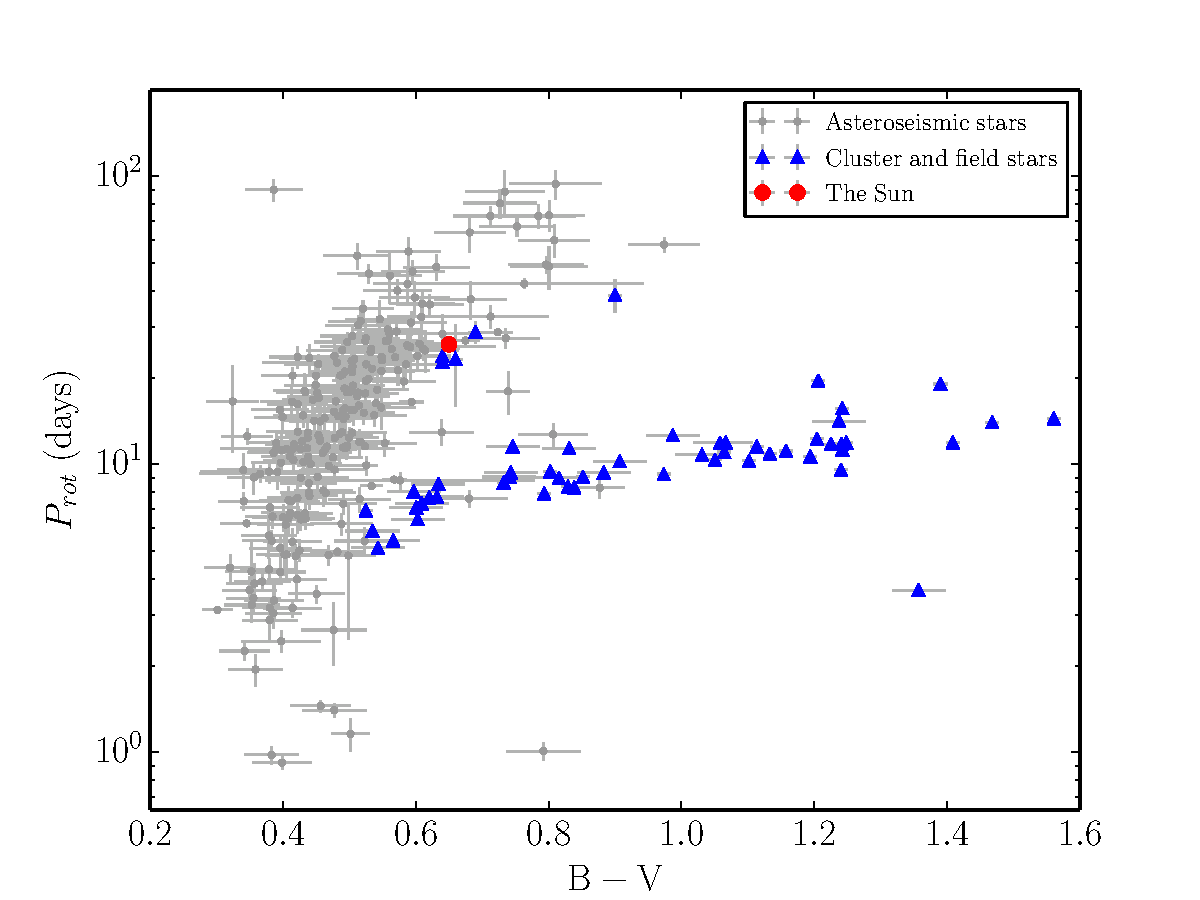
\includegraphics[width=6in, clip=true, trim=0 0 0.5in 0]{/Users/angusr/Python/Gyro/plots/p_vs_bv_paper2.png}
\caption{Photometric rotation period vs B-V colour for \nastero$~$ Kepler targets (black) plus cluster and field stars (blue). The Sun is shown in red.}
\label{fig:3d}
\end{center}
\end{figure}

\begin{figure}[ht]
\begin{center}
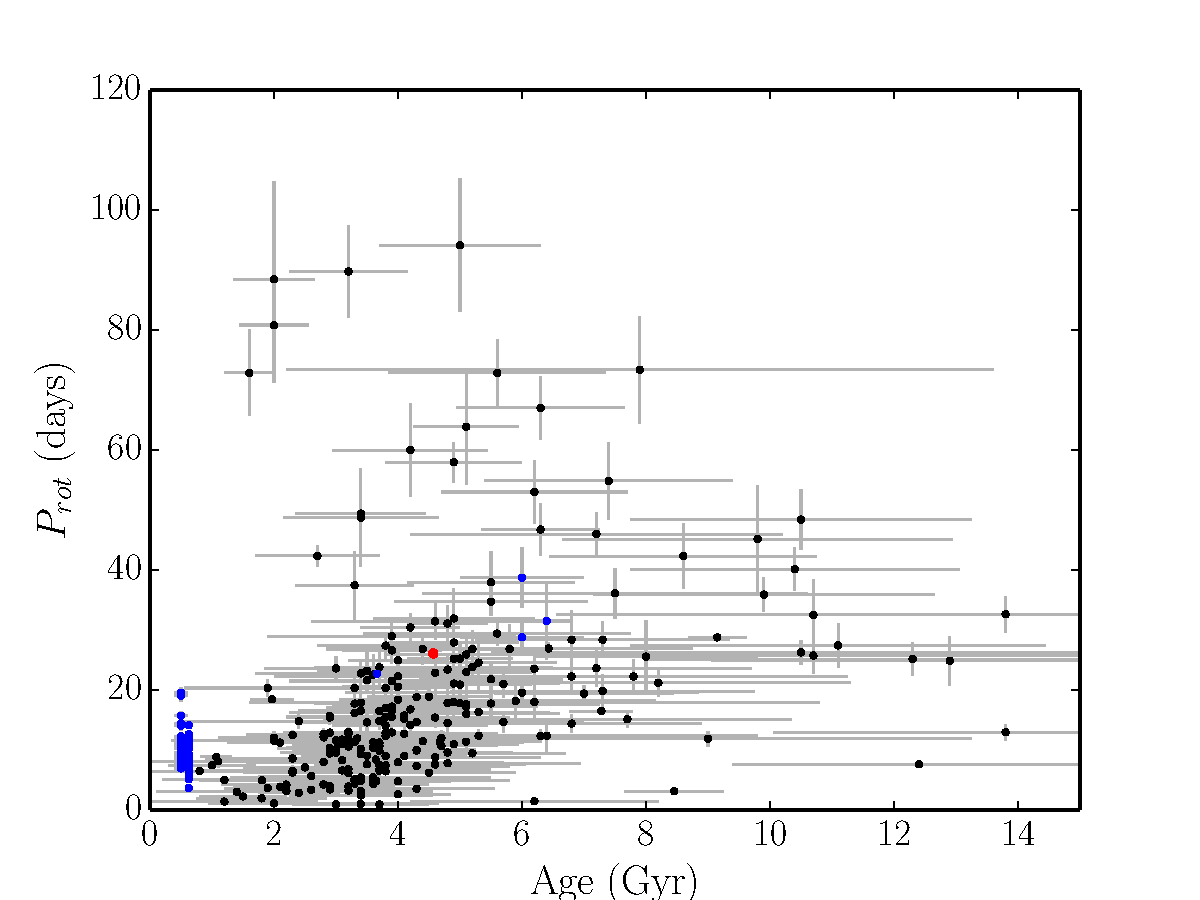
\includegraphics[width=6in, clip=true, trim=0 0 0.5in 0]{/Users/angusr/Python/Gyro/plots/p_vs_a_paper2.png}
\caption{Photometric rotation period vs age for the data described in figure \ref{fig:3d}.}
\label{fig:p_vs_a}
\end{center}
\end{figure}

\begin{figure}[ht]
\begin{center}
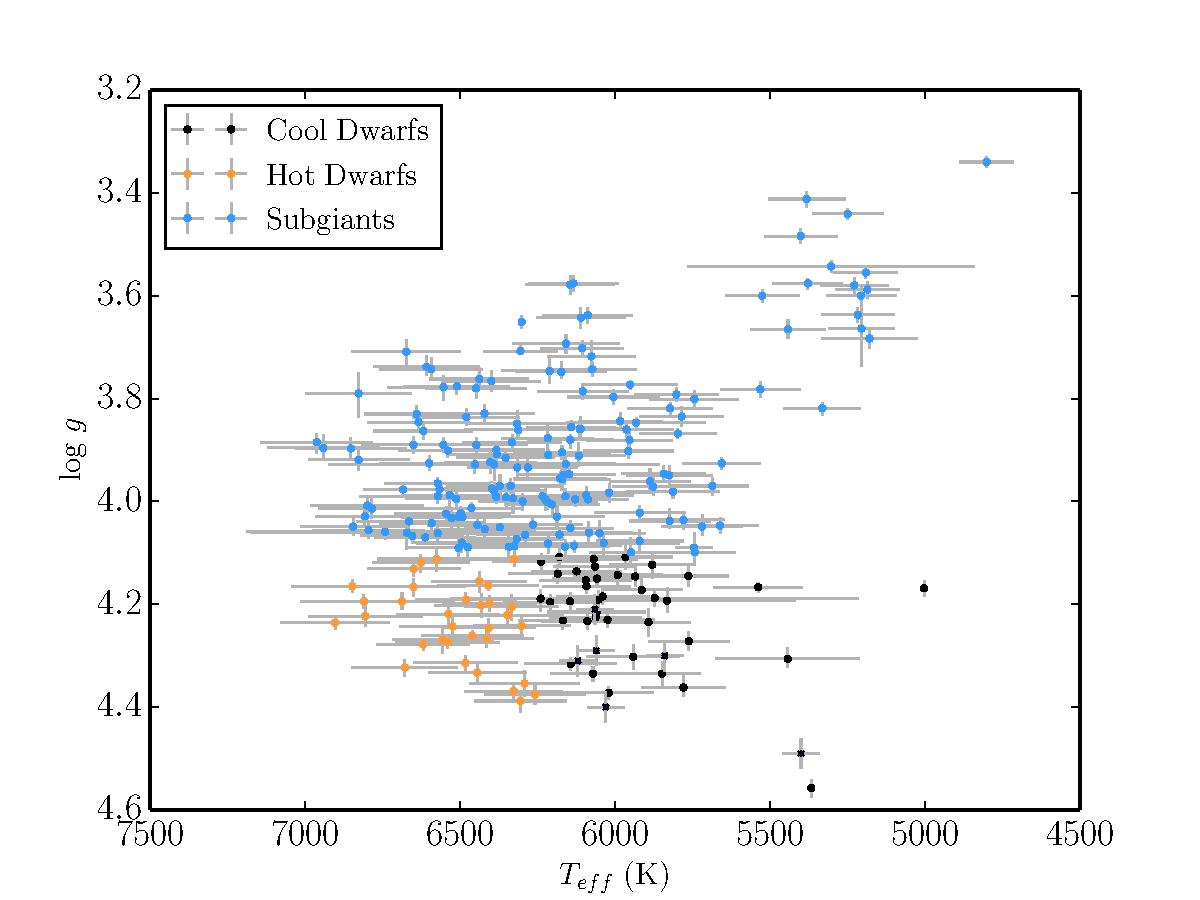
\includegraphics[width=6in, clip=true, trim=0 0 0.5in 0]{/Users/angusr/Python/Gyro/plots/logg_vs_t_paper.png}
\caption{\logg vs \teff for the \nastero asteroseismic stars. Stars with \teff $>$ 6250 K are red and those with \logg $<$ 4.2 are blue. The triangular data points are those with precise ages. Only the black cool dwarfs are expected to follow the gyrochronology relation in equation \ref{eq:Barnes2007_2}.}
\label{fig:p_vs_a}
\end{center}
\end{figure}

\begin{figure}[ht]
\begin{center}
	\subfigure[Coma Berenices and field stars.]{
            \label{fig:CF45}
	    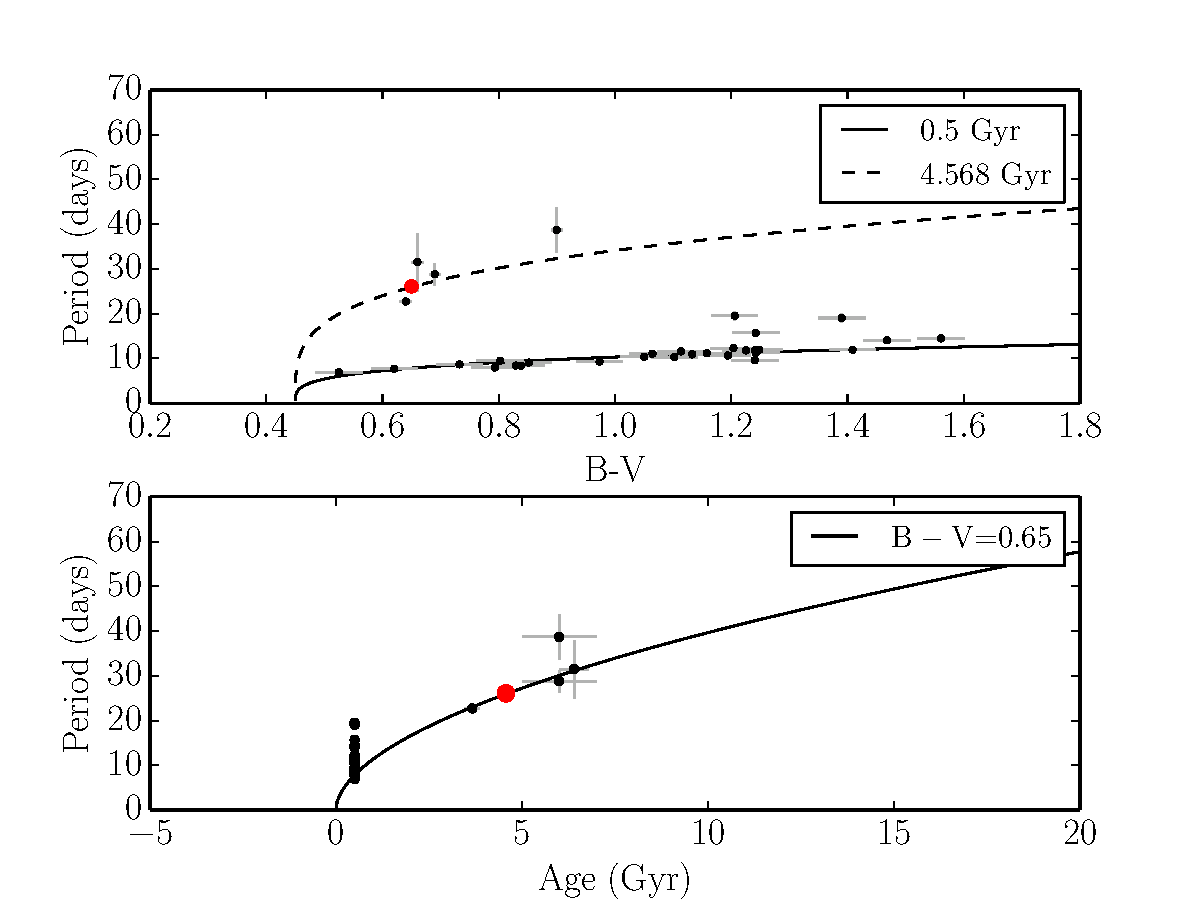
\includegraphics[width=4in, clip=true, trim=0 0 0.5in 0]{/Users/angusr/Python/Gyro/plots/showCF45.png}
        }
	\subfigure[Hyades and field stars.]{
            \label{fig:HF45}
	    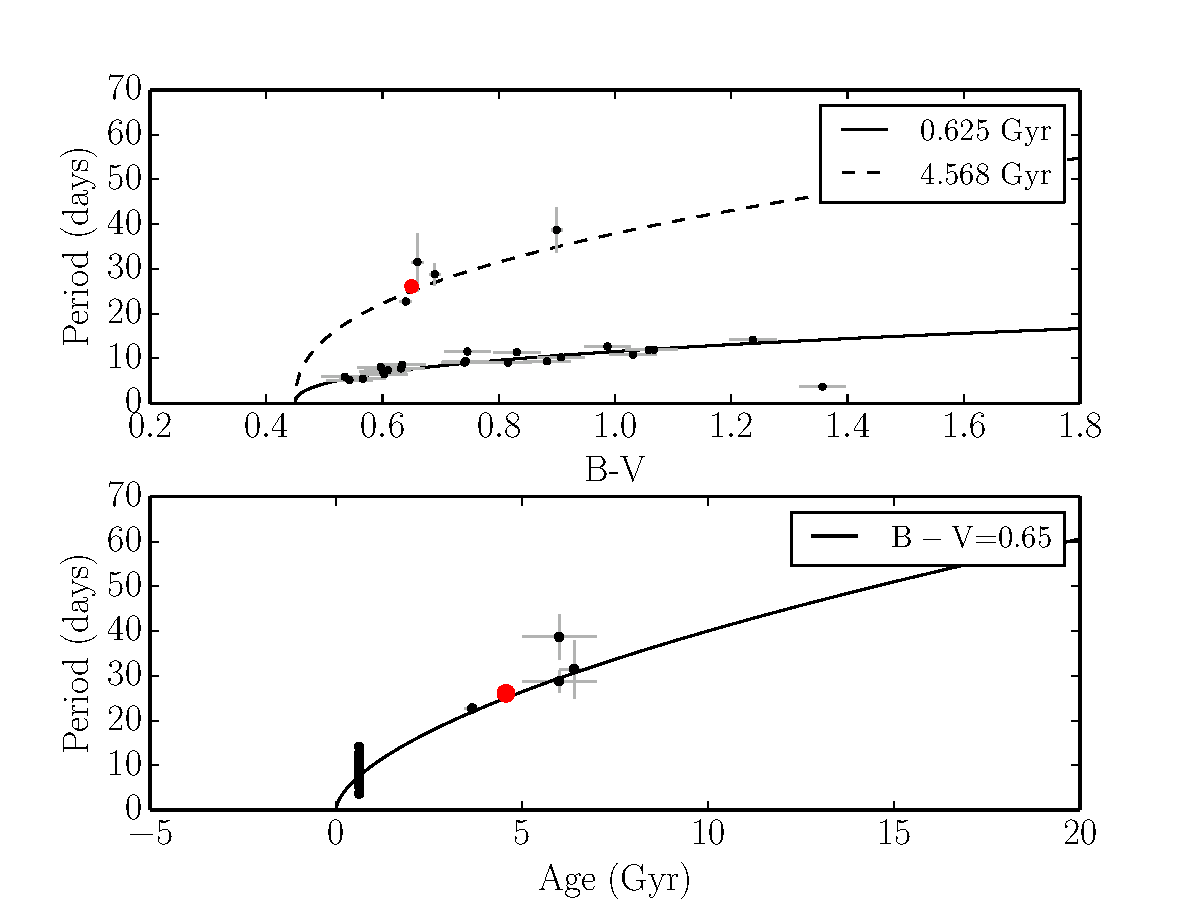
\includegraphics[width=4in, clip=true, trim=0 0 0.5in 0]{/Users/angusr/Python/Gyro/plots/showHF45.png}
        }
    \end{center}
    \caption{ Individual fits to the clusters and field stars. The Sun is the red point. Top panels show period vs B-V with Solar and cluster age isochrones. Bottom panels show period vs age with the period-age relation for a constant B-V value of 0.65 (Solar B-V).}
   \label{fig:subfigures2}
\end{figure}

\begin{figure}[ht]
\begin{center}
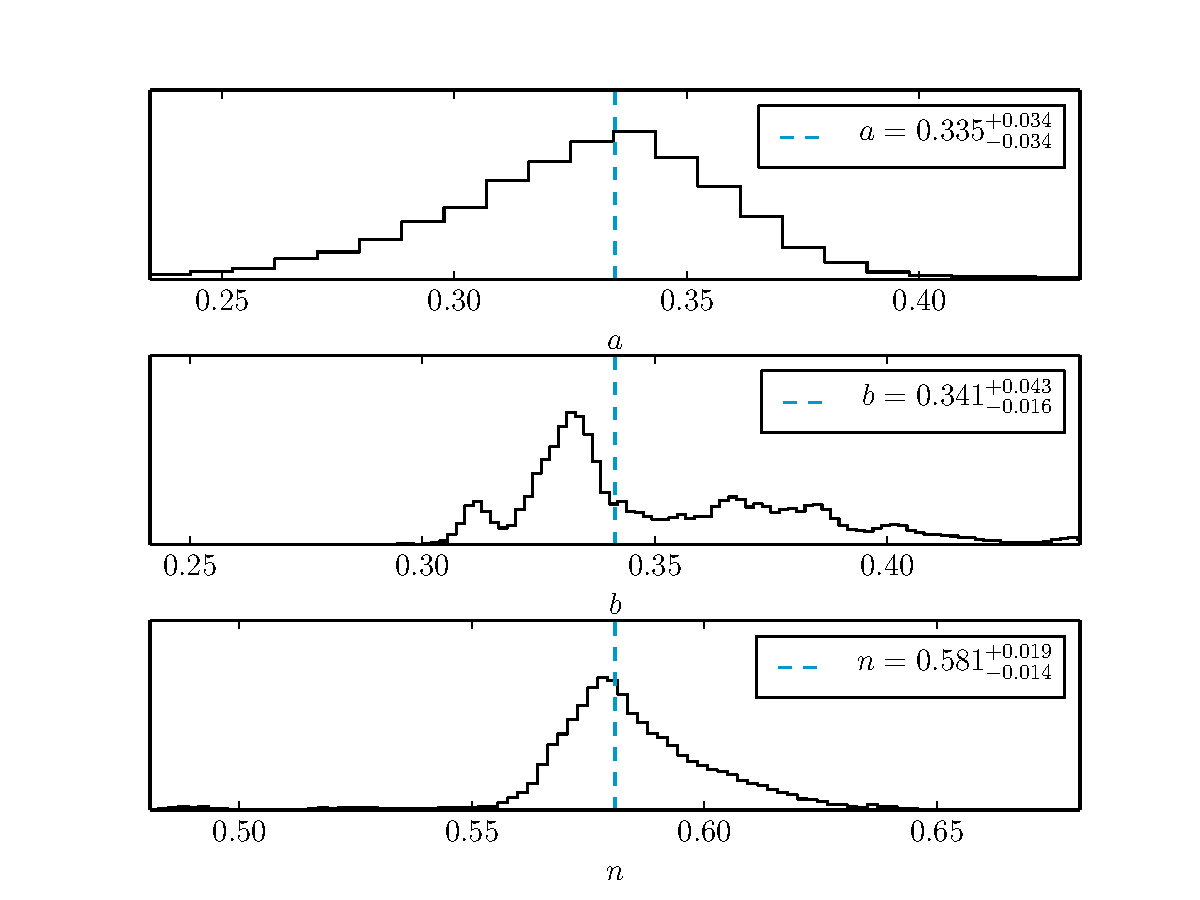
\includegraphics[width=6in, clip=true, trim=0 0 0.5in 0]{/Users/angusr/Python/Gyro/plots/marg_posteriors.png}
\caption{Marginalised posterior PDFs of the three gyrochronology parameters; $a$, $b$ and $n$.}
\label{fig:marg_posteriors}
\end{center}
\end{figure}

\begin{figure}[ht]
\begin{center}
	\subfigure[0.625 Gyr (age of the Hyades)]{
            \label{fig:625}
	    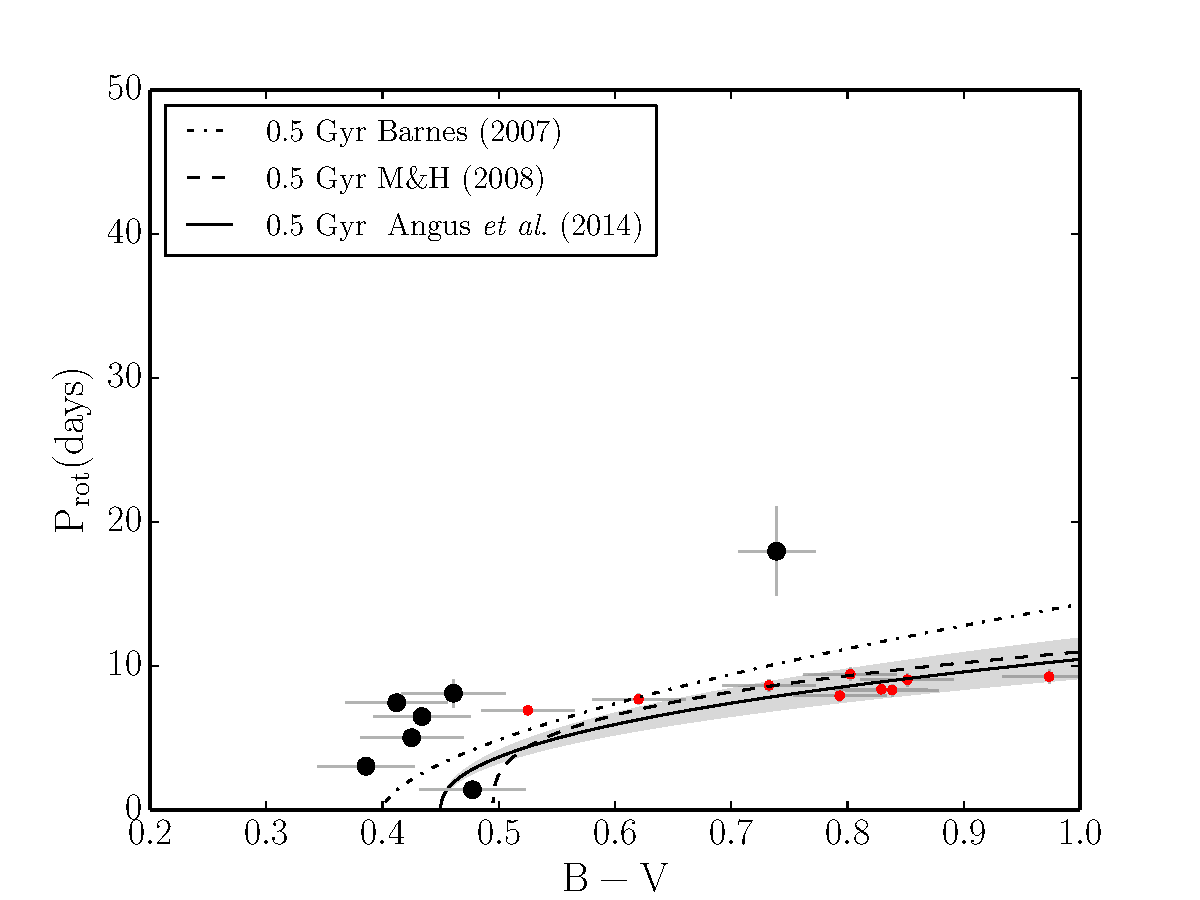
\includegraphics[width=3in, clip=true, trim=0 0 0.5in 0]{/Users/angusr/Python/Gyro/plots/p_vs_bv0.png}
        }
	\subfigure[2 Gyr]{
            \label{fig:2gyr}
	    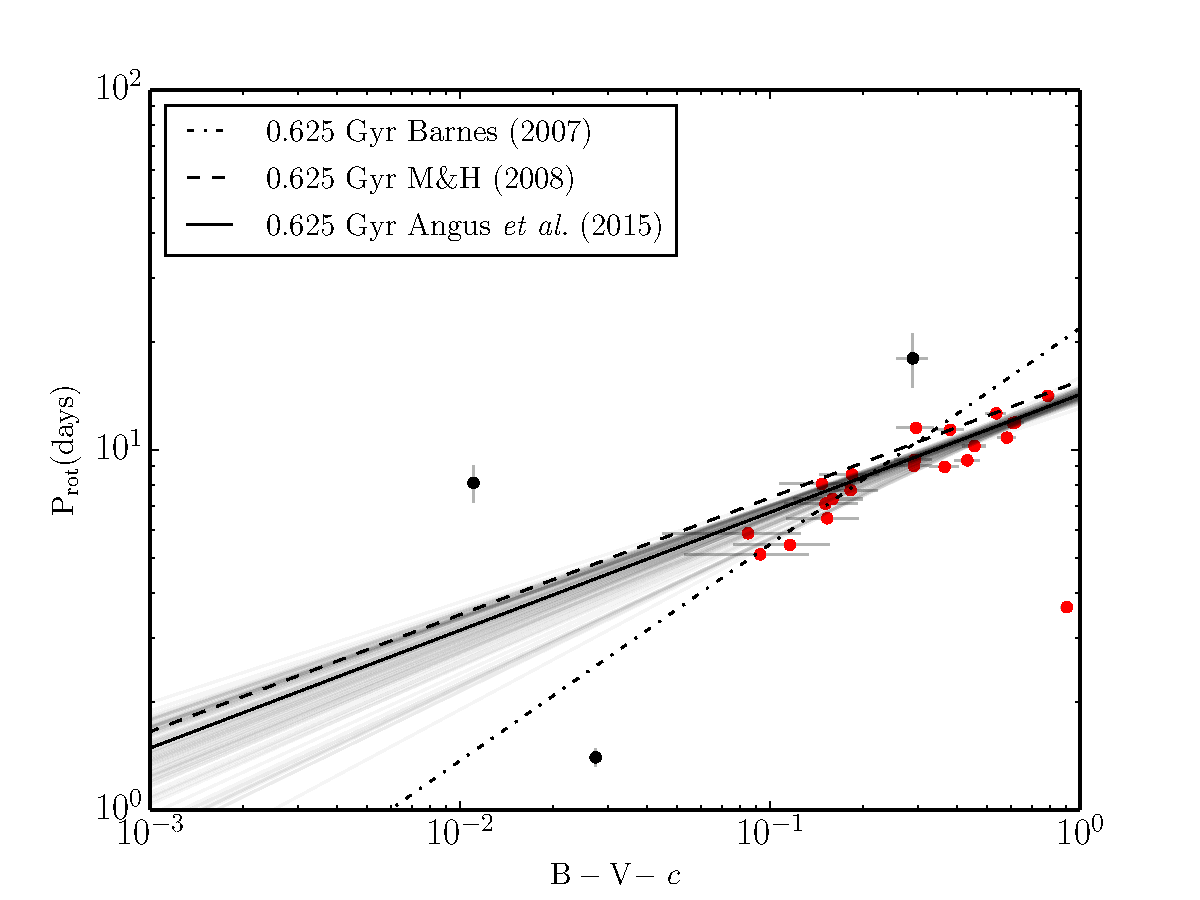
\includegraphics[width=3in, clip=true, trim=0 0 0.5in 0]{/Users/angusr/Python/Gyro/plots/p_vs_bv1.png}
        }
	\subfigure[4.568 Gyr (Solar age)]{
            \label{fig:sungyr}
	    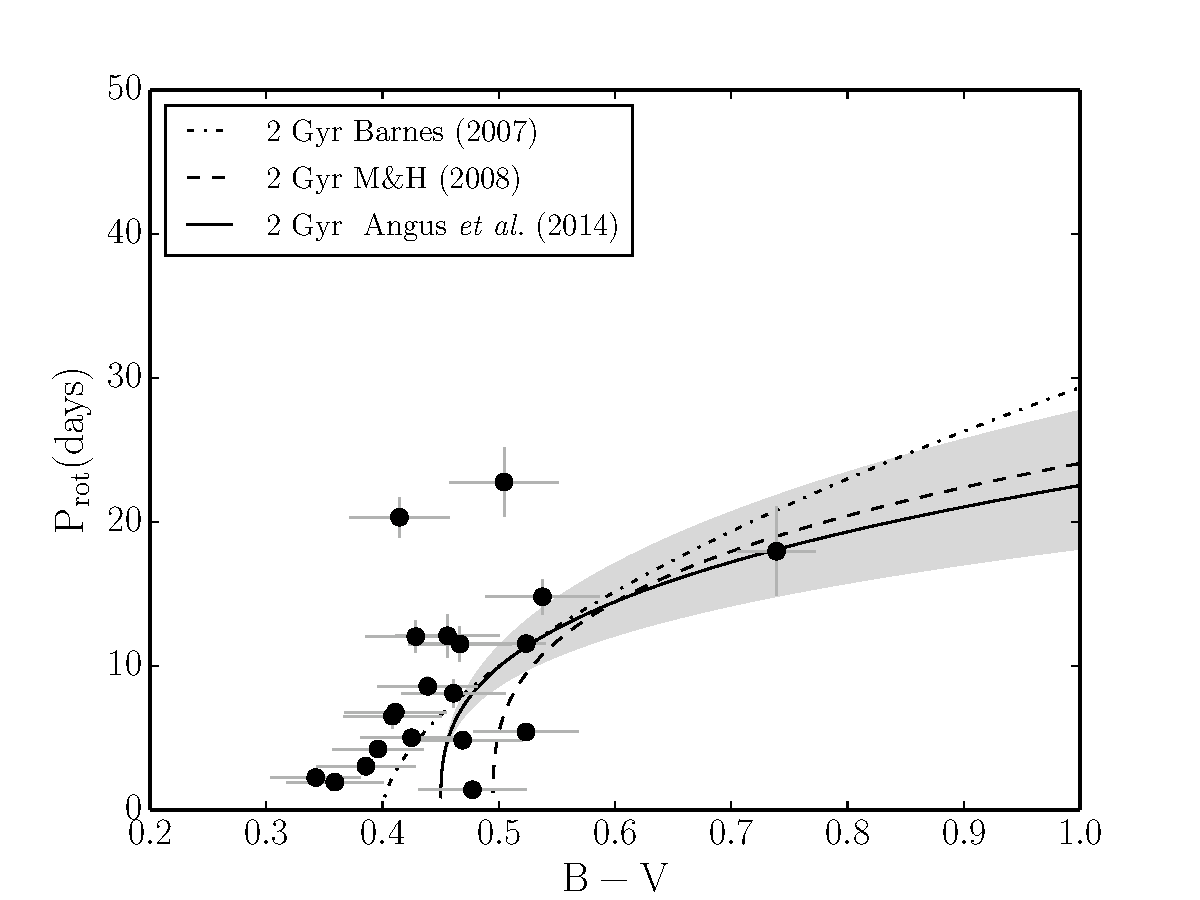
\includegraphics[width=3in, clip=true, trim=0 0 0.5in 0]{/Users/angusr/Python/Gyro/plots/p_vs_bv2.png}
        }
	\subfigure[8 Gyr]{
            \label{fig:8gyr}
	    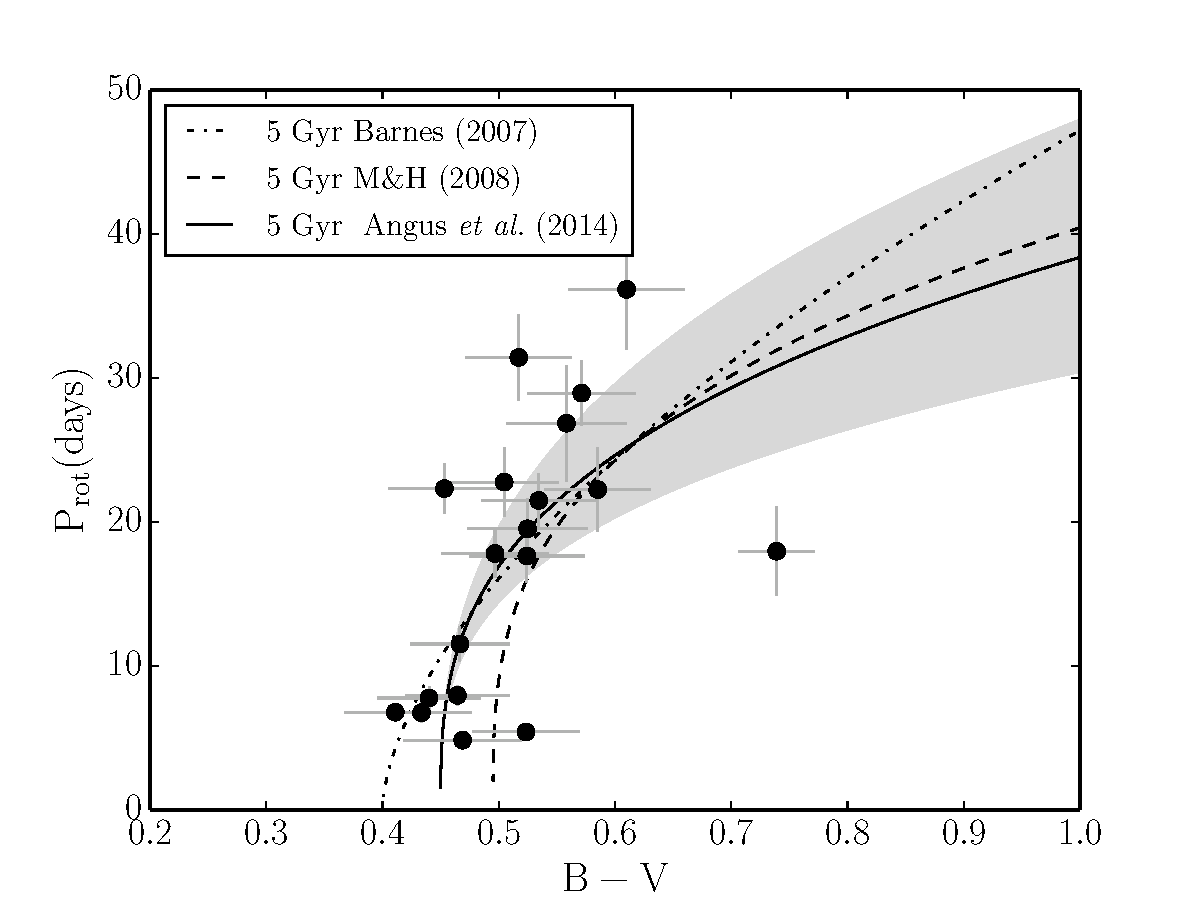
\includegraphics[width=3in, clip=true, trim=0 0 0.5in 0]{/Users/angusr/Python/Gyro/plots/p_vs_bv3.png}
        }
    \end{center}
    \caption{ \prot vs B-V colour for dwarfs within 1$\sigma$ of the reference age with the new gyrochronology relation and \citet{Barnes2007}, and \citet{Mamajek2008} for comparison. Asteroseismic targets are black and cluster and field stars are red. The shaded regions represent the 16th and 84th percentile uncertainties.
     }
   \label{fig:subfigures2}
\end{figure}

\begin{figure}[ht]
\begin{center}
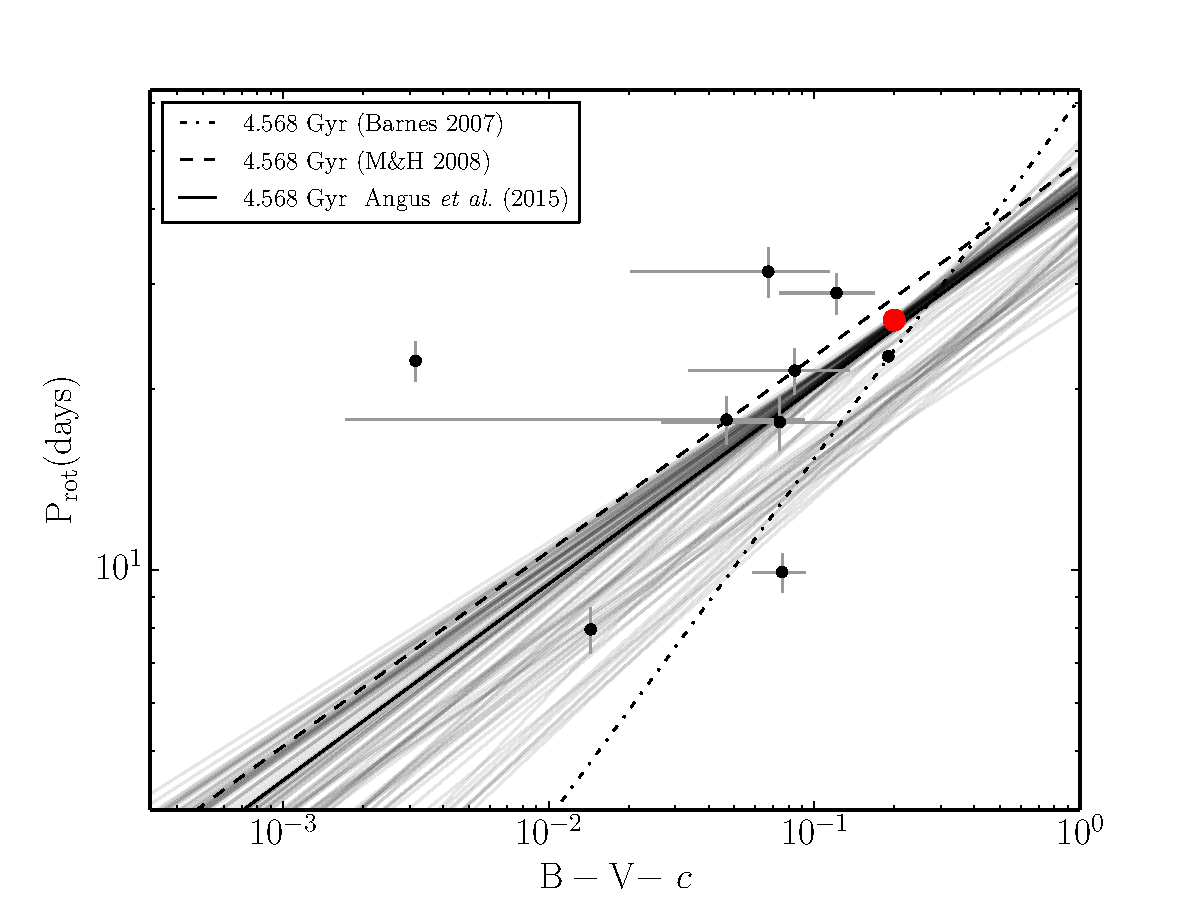
\includegraphics[width=6in, clip=true, trim=0 0 0.5in 0]{/Users/angusr/Python/Gyro/plots/p_vs_bv_solar.png}
\caption{Rotation period vs B-V colour for dwarfs with age within 1$\sigma$ of the Sun's age, 4.568 Gyr. The grey stars are hotter than 6250 K. The Sun is the red point.}
\label{fig:p_vs_bv_solar}
\end{center}
\end{figure}

\begin{figure}[ht]
\begin{center}
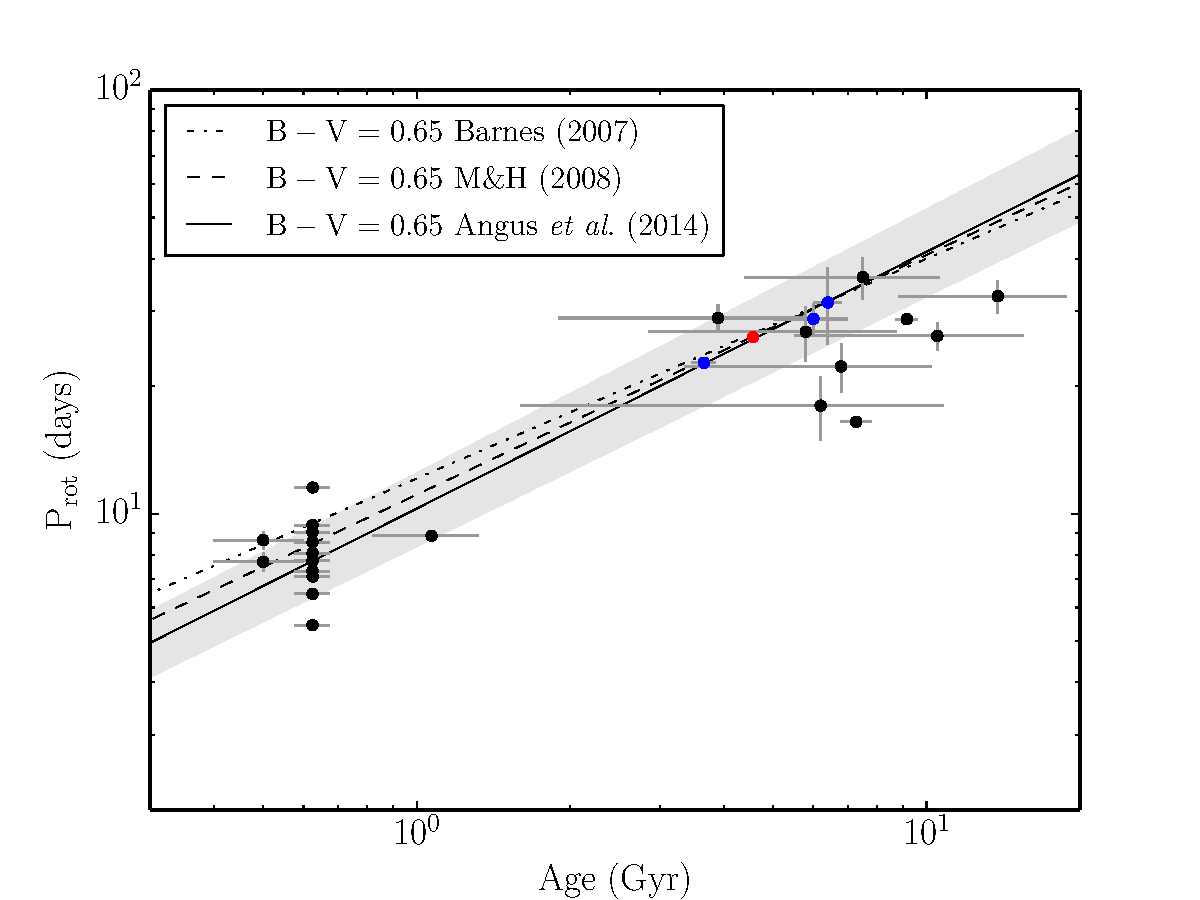
\includegraphics[width=6in, clip=true, trim=0 0 0.5in 0]{/Users/angusr/Python/Gyro/plots/p_vs_a_solar.png}
\caption{Rotation period vs age for cool dwarfs with colour within 10\% of the Sun's: 0.65, with gyrochronology relations of \citet{Barnes2007}, \citet{Mamajek2008} and this work. The shaded region represents the 16th and 84th percentile uncertainties. The Sun is shown in red and the field stars, $\alpha$ Cen A, 18 Sco and 16 Cyg from left to right, are shown in blue.}
\label{fig:p_vs_a_solar}
\end{center}
\end{figure}

\end{document}
